%Dokumententyp
\documentclass[a4paper]{article}


\usepackage[a4paper,left=2cm, right=3cm, top=2cm]{geometry}

%Kodierung
\usepackage[utf8]{inputenc}
\usepackage[T1]{fontenc}

%Grafiken einbinden
\usepackage{graphicx}
\usepackage{subfigure} 

%Position von Grafiken und Tabellen erzwingen:
\usepackage{float}

%URLs im Literaturverzeichnis
\usepackage{url}

\usepackage{amsmath}

%Schriftart Arial:
% \usepackage{helvet}

%Figures with text around it:
\usepackage{wrapfig}

\usepackage{listings}

%seitennummern rechts:
% \usepackage{fancyhdr}
% \fancyhf{} % clear all header and footers
% \renewcommand{\headrulewidth}{0pt} % remove the header rule
% \rfoot{\thepage}
% \fancypagestyle{plain}{%redefining plain pagestyle
% \fancyhf %clear all headers and footers fields
% \fancyhead[R]{\thepage} %prints the page number on the right side of the header
% }

%Schriftart Times New Roman "like"
\usepackage{txfonts}

%Sprache
\usepackage[german]{babel}

%Checkmarks: (usage: \checkmark)
\usepackage{dingbat}

\usepackage{listings}
\usepackage{color}
\definecolor{javared}{rgb}{0.6,0,0} % for strings
\definecolor{javagreen}{rgb}{0.25,0.5,0.35} % comments
\definecolor{javapurple}{rgb}{0.5,0,0.35} % keywords
\definecolor{javadocblue}{rgb}{0.25,0.35,0.75} % javadoc
 
\lstset{language=Java,
basicstyle=\ttfamily,
keywordstyle=\color{javapurple}\bfseries,
stringstyle=\color{javared},
commentstyle=\color{javagreen},
morecomment=[s][\color{javadocblue}]{/**}{*/},
numbers=left,
numberstyle=\tiny\color{black},
stepnumber=1,
numbersep=5pt,
tabsize=4,
showspaces=false,
lineskip={-1.5pt},
showstringspaces=false}

%Tabellenextras
\usepackage{tabularx}

%Zeilenabstand 1.5
\linespread{1.5}
\usepackage{setspace}

%Figure Captions mit Fußnoten
\usepackage{footnote}
%\setlength{\parindent}{0pt} 


%itemize items richtig ausrichten (nicht links überlappen!)
% \setlist{leftmargin=0}

% %%%%TITELSEITE%%%%%%(
% \title{ Konzept und Implementierung\\ eines Systems zur \\Anforderung und Verwaltung von virtuellen privaten Clustern}
% \author{\textbf{\large Bachelorarbeit}}
% 
% \date{zur Erlangung des akademischen Grades Bachelor of Science an der Universität Paderborn im Fachbereich Informatik im Studiengang Bachelor Informatik}

% %%%%TITELSEITE%%%%%%)

% \pagestyle{fancy}
\begin{document}

\title{Algorithmische Geometrie - Sommersemester 2015\\
       5. Aufgabenblatt }
\author{Simon Koennecke und Felix Bröker}
\date{}
\maketitle

\section*{Aufgabe 1 - Suchen in ebenen Unterteilungen}
\subsection*{Aufbau einer Datenstruktur}
Annahme: Es ist der normalisierte ebene Graph $G$ gegeben. 

Wir konstruieren im Folgenden auf Basis von $G$ eine Directed Acyclic Graph-Struktur $S$, mittels derer 
später in $\mathcal{O}(\log n)$ ermittelt werden kann, in welcher Facette/Dreieck des Graphen
sich ein Punkt $p$ befindet:

$S_i$ sei die Triangulierung der verbliebenen Punkte vom Graphen $G$ im Verarbeitungsschritt $i$, wobei
zu Beginn gilt: $S_0$ = $G$.

\begin{enumerate}
 \item Solange $S_i$ kein Dreieck
 \begin{enumerate}
  \item Setze $S_{i+1} = S_i$
  \item Finde eine unabhängige Knotenmenge $U_i$ von $S_i$, wobei jeder Knoten der Menge Grad $< 12$ besitzt.
  \item Solange $U_i$ nicht leer
  \begin{enumerate}
   \item Enferne beliebigen Knoten $u \in U_i$ aus $S_{i+1}$. Benenne die hiermit entfallenen Dreiecke als $\Delta_{alt}$
   \item Trianguliere die Nachbarschaft von $u$ in $S_{i+1}$ neu. Benenne die neu entstandenen Dreiecke als $\Delta_{neu}$.
   \item Die Verbindungen zwischen $S_i$ und $S_{i+1}$ werden entsprechend der Kantenmenge
   
   $\left\{(e_{neu}, e_{alt}) \quad|\quad (e_{neu} \in \Delta_{neu}, e_{alt} \in \Delta_{alt} \right\}$ konstruiert.
  \end{enumerate}
  \item Setze $i = i + 1$
 \end{enumerate}

\end{enumerate}


\section*{Aufgabe 2 - $L_1$-Voronoi-Diagramme}

\begin{figure} [htbp] 
    \subfigure[Voronoi-Diagramm (Manhattan-Distance) - Beispiel 1]{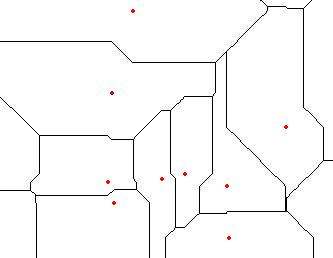
\includegraphics[width=0.5\textwidth]{01.jpg}} 
    \subfigure[Voronoi-Diagramm (Manhattan-Distance) - Beispiel 2]{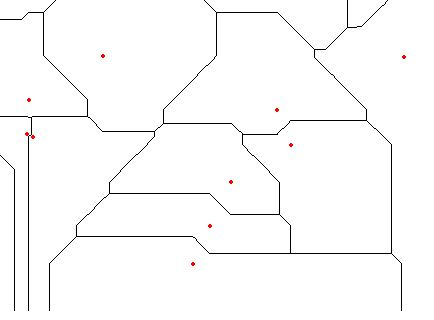
\includegraphics[width=0.5\textwidth]{02.jpg}} 
    \subfigure[Voronoi-Diagramm (Manhattan-Distance) - Beispiel 3]{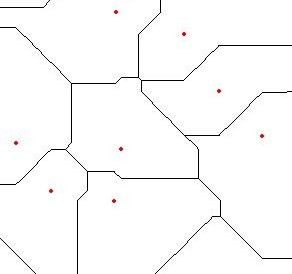
\includegraphics[width=0.5\textwidth]{03.jpg}} 
%\caption{} 
\end{figure} 

\section*{Aufgabe 3 - Suche in ebenen Unterteilungen - Verallgemeinerung}





\end{document}
